\documentclass[a5paper,12pt,titlepage]{article}
\usepackage{kantlipsum}
\usepackage{geometry}
% \usepackage{showframe}
\usepackage{graphicx}
\usepackage{changepage}
\usepackage{tikzpagenodes}
\usepackage{tabularx}
\usepackage{tikz}
\usetikzlibrary{calc}
\usetikzlibrary{decorations.pathmorphing}

\usepackage{fontspec}
\usepackage{hyperref}
\usepackage{microtype}
\setmainfont{Adobe Garamond Pro}

\geometry{top=1in, bottom=1in, left=2cm, right=2cm}

\setlength{\parindent}{0pt}

\begin{document}
% \maketitle

\begin{titlepage}
    \centering

    \begin{tikzpicture}[remember picture,overlay,
        shift={(current page.north)}
    ]
    \node[anchor=north,xshift=0,yshift=-1.25cm]{\includegraphics[width=0.6\paperwidth]{Us}};
    \end{tikzpicture}

    % \begin{tikzpicture}[remember picture,overlay,
    %     shift={(current page.north west)}
    % ]
    % \node[anchor=north west,xshift=0.65cm,yshift=-0.65cm]{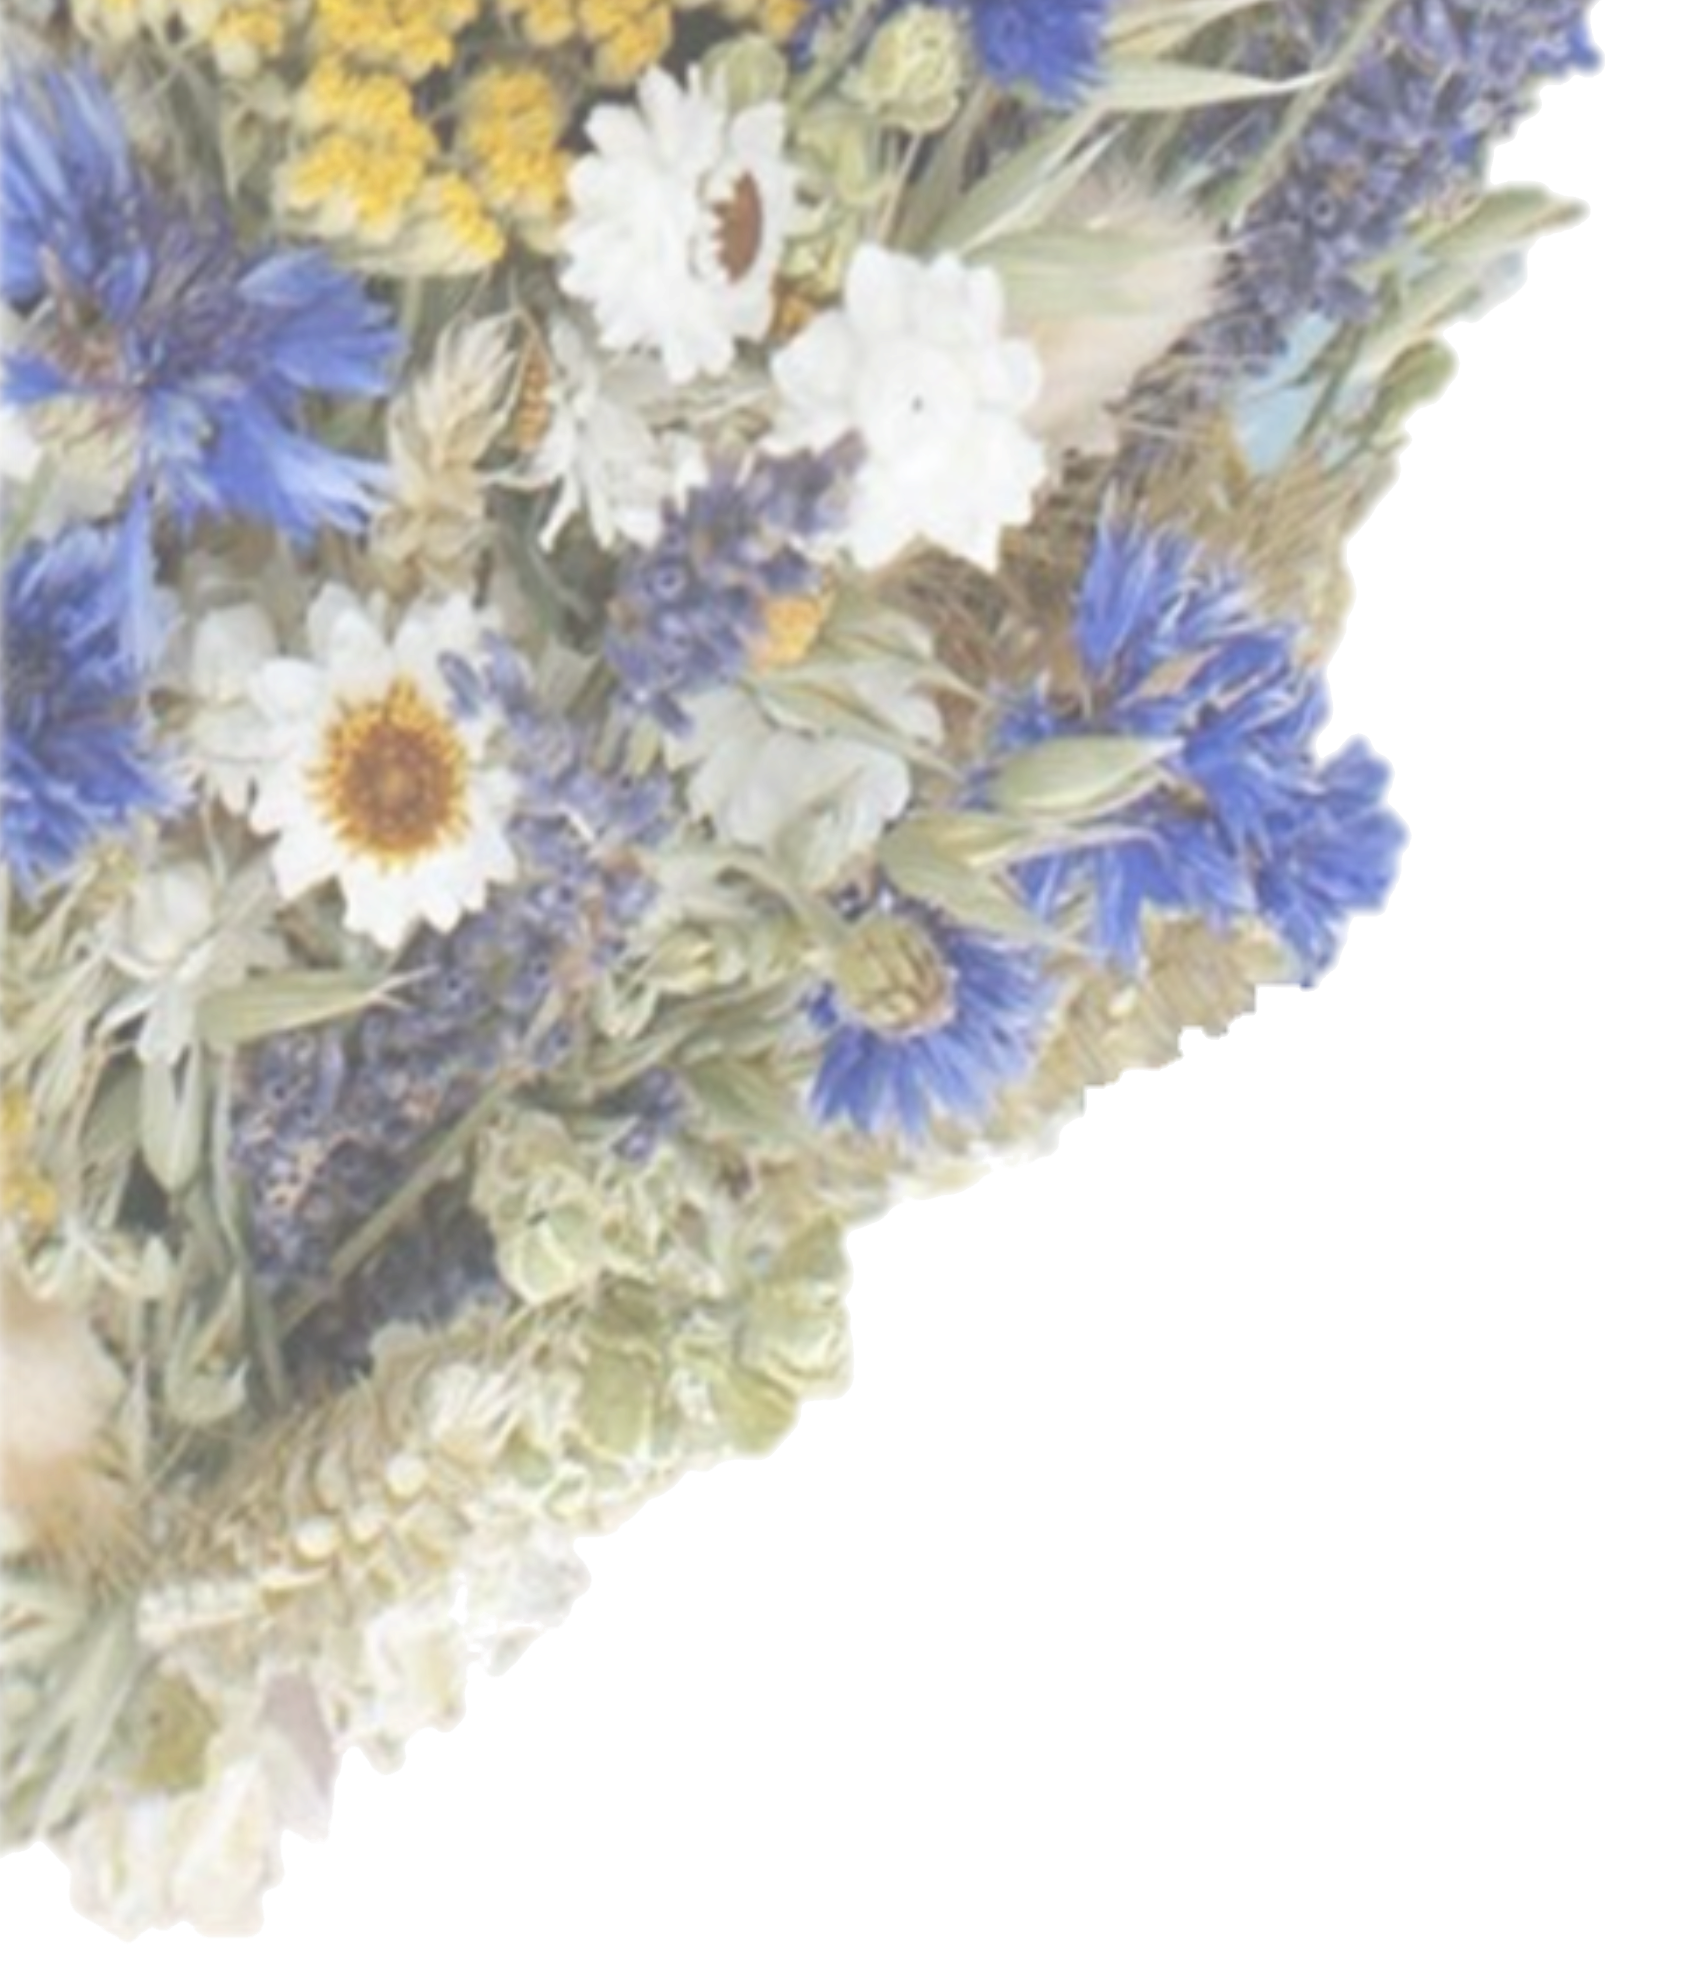
\includegraphics[width=0.3\paperwidth]{bouquet_edit3_transparent}};
    % \end{tikzpicture}

    % \begin{tikzpicture}[remember picture,overlay,
    %     shift={(current page.north east)}
    % ]
    % \node[xscale=-1,anchor=north west,xshift=0.65cm,yshift=-0.65cm]{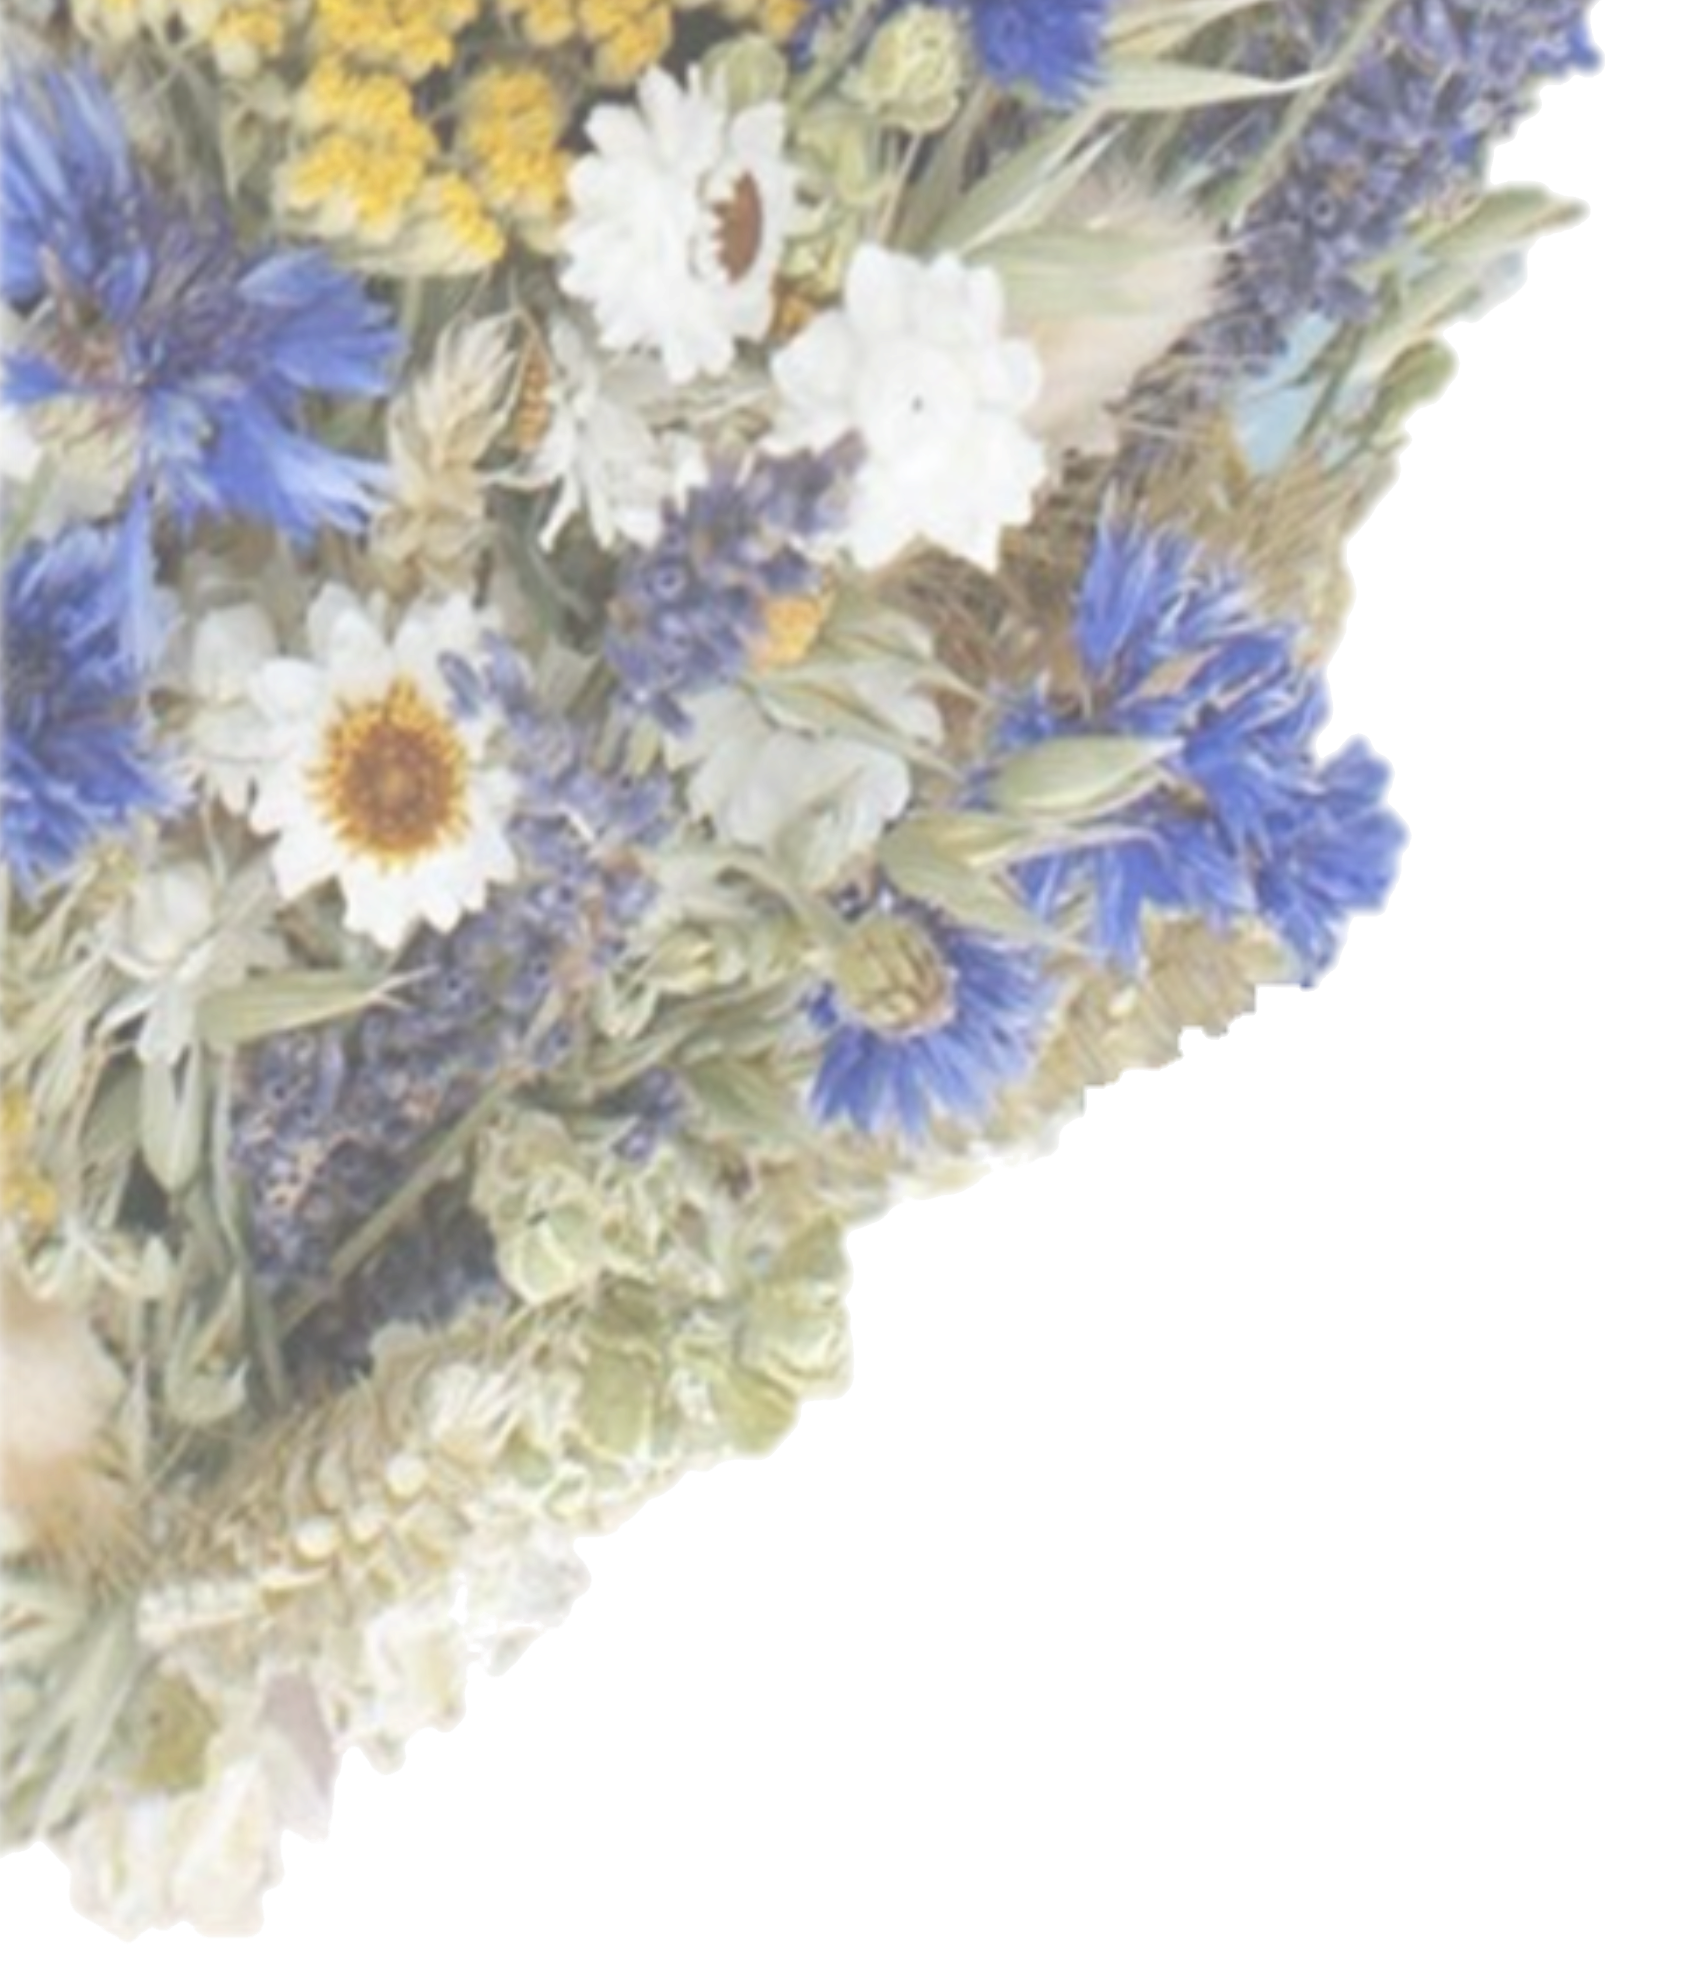
\includegraphics[width=0.3\paperwidth]{bouquet_edit3_transparent}};
    % \end{tikzpicture}

    \begin{tikzpicture}[overlay,remember picture]
        \draw [line width=0.3mm,draw=black]
            ($ (current page.north west) + (0.6cm,-0.6cm) $)
            rectangle
            ($ (current page.south east) + (-0.6cm,0.6cm) $);
        \draw [line width=0.2mm,draw=black]
            ($ (current page.north west) + (0.8cm,-0.8cm) $)
            rectangle
            ($ (current page.south east) + (-0.8cm,0.8cm) $);
    \end{tikzpicture}
    
        
    \centering
    \vspace*{7cm}
    \begin{adjustwidth}{-2cm}{-2cm}
    \centering
    {\LARGE The Blessing of Marriage of\\[1em]Dr. Rebecca Claire\\{\em and}\\ Mr. Adam Alexander \\[1em]{Brouwers-Harries}\par}
    \end{adjustwidth}
	\vspace{\fill}
    {\large The Stables, Prestonfield House\par}
    {\large Rev.~Peter Harris\par}
    % \vspace{2.5cm}
    {\large September 10th, 2022\par}
    \vspace{-2em}
	% \vspace{2cm}
    
\end{titlepage}

\hspace{2em}Welcome to this blessing of our marriage, and our rather belated wedding reception! We're so glad to be able to gather with you all today and properly celebrate our marriage, even though it's been almost two years since we officially tied the knot. We're grateful to all of you for joining us, and thankful that you're able to make time to be with us today.

\hspace{2em}Although the impact of COVID-19 has now reduced to the point where we feel comfortable holding a `big' party, we would like to remind you all to take reasonable precautions, and respect the precautions taken by others. We will not be masking {\em by default}, but if anybody near to you asks that you put on a mask, please comply with their wishes. Additionally, if you test positive in the coming days after the party please contact us {\em at once} so that we can notify other guests.

\hspace{2em}Finally, as we have already had plenty of `proper' photos taken at our original wedding (and to avoid the stress of more!) we have elected not to engage the services of a professional photographer for our party. Please feel free to take photos and videos throughout the day and evening, and either send them to us directly, or post them on social media with the hashtag:{\begin{center}\large \texttt{\#BrouwersHarries22} \end{center}} If you are not comfortable with pictures of you appearing on social media, please let us know and we will direct others to take down or avoid uploading photos of you.

\hspace{2em}We hope you have a wonderful time today,

\begin{flushright}
Rebecca \& Adam
\end{flushright}

% \vspace*{\fill}
\clearpage

\section{Schedule}
\begin{table}[h!]
\begin{center}
    \begin{tabular}{ l c r } 
    %  \hline
{\em 1:30pm} & \hspace{5em} & Guests begin to arrive \\[5pt]
{\em 2pm} & \hspace{5em} & Blessing and renewal of vows \\[5pt]
{\em 2:30pm} & \hspace{5em} & Drinks reception \\[5pt]
{\em 3:15pm} & \hspace{5em} & Swing dance taster (in the stables) \\[5pt]
{\em 4pm} & \hspace{5em} & Take seats for dinner \\[5pt]
{\em 4:30pm} & \hspace{5em} & Speeches \& Cutting of the cake \\[5pt]
{\em 5pm} & \hspace{5em} & Dinner \\[5pt]
{\em 8pm} & \hspace{5em} & First dance \& live music begins \\[5pt]
{\em 10pm} & \hspace{5em} & Evening food \\[5pt]
{\em 1am} & \hspace{5em} & Guests leave \\
    %  \hline
    \end{tabular}
\end{center}
\end{table}

\clearpage

\section{Wedding Blessing} 

The grace of our Lord Jesus Christ, the love of God, and the fellowship of the Holy Spirit be with you all. \\

We gather here to give thanks and to rejoice together with Rebecca and Adam as they celebrate their wedding and seek God's blessing on them. \\

The Church declares that\\

Marriage is a gift of God in creation\\
and a means of his grace;\\
it is given that a husband and wife\\
may comfort and help each other,\\
living faithfully together\\
in times of need as well as in plenty,\\
in sadness and in joy,\\
in sickness and in health;\\
it is given that with delight and tenderness\\
they may know each other in love.\\

\vspace{1em}
In marriage a couple join together in a covenant relationship just as Christ joins with his Bride the church.\\
Therefore we pray that, strengthened and guided by God, Rebecca and Adam may continue to fulfil his purpose for their life together.\\


\clearpage

\section{An adaptation of 1\textsuperscript{st} Corinthians 13}

\textsuperscript{\em 1} If I speak in the tongues of men or of angels, but do not have love, I am only a resounding gong or a clanging cymbal.\\[0.25em]

\textsuperscript{\em 2} If I have the gift of prophecy and can fathom all mysteries and all knowledge, and if I have a faith that can move mountains, but I do not have love, I am nothing. \\[0.25em]

\textsuperscript{\em 3} If I give all I possess to the poor and sacrifice my body to hardship that I may boast, but do not have love, I gain nothing. \\[0.25em]

\textsuperscript{\em 4} Love is patient, love is kind. It does not envy, it does not boast, it is not proud. \\[0.25em] 

\textsuperscript{\em 5} It does not dishonor others, it is not self-seeking, it is not easily angered, it keeps no record of wrongs. \\[0.25em] 

\textsuperscript{\em 6} Love does not delight in evil but rejoices with the truth. \\[0.25em] 

\textsuperscript{\em 7} It always protects, always trusts, always hopes, always perseveres. \\[0.25em]

\textsuperscript{\em 8} Love never fails. At the end of all things three things will remain: faith, hope and love. But the greatest of these is love. \\[0.25em]


\clearpage 


\section{Renewal of Wedding Vows}

{\em The minister says}\\
{\bf

\hspace{2em} On your wedding day

\hspace{2em} you promised to love each other

\hspace{2em} as Husband and Wife

\hspace{2em} to have and to hold

\hspace{2em} from that day forward,

\hspace{2em} for better, for worse,

\hspace{2em} for richer, for poorer,

\hspace{2em} in sickness and in health,

\hspace{2em} to love and to cherish,

\hspace{2em} till death you do part,\\
}

Now today, in the presence of your family and friends, do you affirm and renew this vow.\\

{\em Rebecca and Adam:} 

\hspace{2em} {\bf I do}\\

{\em The minister says to the congregation}\\

\hspace{2em} Will you, the family and friends of Rebecca and Adam continue to support and uphold them in their lives together and in the days to come?\\

\hspace{2em} {\bf We will.}

\clearpage

\section{Prayers}

Loving lord, we thank you for Rebecca and Adam, we thank you that they have found such love, faith and trust in each other.\\

Throughout all the chances and changes of life, help them to be forever loving and ever true to each other.\\

Bless them and watch over them, and all their family and friends. \\

Guard them from the troubles of life that can destroy our love. And when times of trial come grant them the strength and wisdom to face each day and be drawn closer to each other, and closer to you O Lord.\\

\section{Closing Blessing}

May your life in this world be a happy one\\

May the sun be warm and may the skies be blue. \\

May each storm that comes your way clear the air for a brighter day. \\ 

May the saints and Saviour watch over you, \\[0.25em]

And the blessing of God Father, Son, and Holy Spirit be with you and remain with you now and always.\\

{\bf Amen.}

\clearpage

{\bf Thanks:}

\hspace{2em} We'd like to thank a few important people for helping to make our wedding happen, and supporting us along the way.


\hspace{2em} Firstly, of course, we'd like to thank those at the Church who have had such key roles in the ceremony: Rev.~Nick Wills, our Rector, Sheila Chisholm, the Organist, and Liz for assistance with the church flowers. 


\hspace{2em} We would also like to thank Chris Harries for agreeing to be the Best Man (and signing the schedule), Ayden Brouwers for his excellent reading, and Melanie Jutton for her unerring support, and for also being a signatory of the schedule. 

\hspace{2em} Our orignial conception of a socially distanced reception, and our restricted family reception, would not be possible without the assistance of Mary-Jane Brouwers, as well as Hugh, who also very kindly provided his car as our wedding carriage. 

\hspace{2em} Finally, we would like to thank all of you for attending, despite the danger that this brings to some of you, and for helping us to stay safe while celebrating our love in these turbulent times. 

\vspace{\fill}

\begin{center}
{\tiny \LaTeX \hspace{0.05em} source available upon request.}

\end{center}


\end{document}